\chapter{VIABILIDADE FINANCEIRA}

Este capítulo apresenta uma visão geral dos custos envolvidos no desenvolvimento do sistema, detalhando os gastos com infraestrutura, equipe e ferramentas, além da receita gerada. Também são descritos três cenários financeiros (realista, otimista e pessimista), permitindo visualizar os riscos e oportunidades relacionados ao investimento.

Por se tratar de um projeto acadêmico em que não houve custos nem retorno financeiro de fato, cada seção do capítulo foi analisada com base em valores estimados através de pesquisas realizadas pela equipe. Ao todo, são feitas duas análises diferentes: uma considerando que o projeto será entregue para um cliente específico (a entidade parceira do projeto) e a outra em um eventual \gls{saas}.

\section{Custos}

\label{sec:custos}

A Tabela \ref{tab:custo-mensal-projeto} apresenta os custos com mão de obra, infraestrutura e ferramentas aplicadas no desenvolvimento do projeto.

\begin{table}[htbp]
	\centering
	\caption{Custos mensais estimados do projeto}
	\label{tab:custo-mensal-projeto}
	\begin{tabular}{lrr}
		\toprule
		\textbf{Item de Custo} & \textbf{Valor Unitário (R\$)} & \textbf{Valor Total (R\$)} \\
		\midrule
		\multicolumn{3}{l}{\textbf{Mão de Obra}} \\
		\quad Gestor & 1.250,00 & 1.250,00 \\
		\quad Tech Lead & 2.000,00 & 2.000,00 \\
		\quad Desenvolvedor Fullstack (3x) & 750,00 & 2.250,00 \\
		\quad Auditora Técnica & 500,00 & 500,00 \\
		\cmidrule{3-3}
		\multicolumn{2}{l}{\textbf{Subtotal Mão de Obra}} & \textbf{6.000,00} \\
		\midrule
		\multicolumn{3}{l}{\textbf{Infraestrutura e Ferramentas}} \\
		\quad AWS EC2 (múltiplas instâncias) & --- & 250,00 \\
		\quad Internet (banda larga) & --- & 120,00 \\
		\quad Consumo elétrico (6 computadores) & --- & 40,00 \\
		\quad SonarQube (licença comercial) & --- & 350,00 \\
		\quad Notion Plus (equipe) & --- & 400,00 \\
		\quad Figma Professional (acesso full + dev) & --- & 160,00 \\
		\cmidrule{3-3}
		\multicolumn{2}{l}{\textbf{Subtotal Infraestrutura}} & \textbf{1.320,00} \\
		\midrule
		\multicolumn{2}{l}{\textbf{TOTAL MENSAL}} & \textbf{7.320,00} \\
		\bottomrule
	\end{tabular}
	\fonte{Produzido pelos autores}
\end{table}

Para determinar os custos da mão de obra, utilizou-se a plataforma \emph{Glassdoor} \cite{glassdoor-2025}. Nela, pesquisou-se o salário médio de cada um dos cargos definidos na subseção \ref{subsec:papeis-equipe} considerando a cidade de São Paulo.

Conforme aconselhado pelo orientador do projeto, considerou-se um dia de trabalho inteiro equivalente a apenas uma hora para se aproximar da disponibilidade real que os membros da equipe podiam dedicar ao desenvolvimento do projeto. Assim, o custo mensal de cada cargo foi obtido considerando o valor da hora trabalhada.

O preço da infraestrutura das instâncias \gls{ec2}, operando 24 horas por dia, foi calculado utilizando a própria calculadora de preços da \gls{aws} \cite{aws-calculadora-2025}. Já o custo de internet foi baseado numa média de preços online \cite{internet-precos-2025}, enquanto o de consumo elétrico considerou a tarifa residencial da cidade de São Paulo no ano de 2024 \cite{enel-tarifa-2024} para 6 computadores com um consumo médio de 300 W por hora.

Quanto às ferramentas utilizadas no projeto, levou-se em conta os preços do \emph{SonarQube} \cite{sonarqube-preco-2025}, as mensalidades do \emph{Notion} \cite{notion-preco-2025} e os planos do \emph{Figma} \cite{figma-preco-2025}. Os valores em dólar foram convertidos considerando uma cotação média de R\$ 5,50 em junho de 2025.

A Tabela \ref{tab:custo-total-projeto} apresenta o custo total do projeto considerando os 9 meses de desenvolvimento previstos na Seção \ref{sec:duracao}.

\begin{table}[htbp]
	\centering
	\caption{Custos totais do projeto}
	\label{tab:custo-total-projeto}
	\begin{tabular}{lrr}
		\toprule
		\textbf{Item de Custo} & \textbf{Valor Mensal (R\$)} & \textbf{Valor Total (R\$)} \\
		\midrule
		\multicolumn{3}{l}{\textbf{Mão de Obra}} \\
		\quad Gestor & 1.250,00 & 11.250,00 \\
		\quad Tech Lead & 2.000,00 & 18.000,00 \\
		\quad Desenvolvedor Fullstack (3x) & 2.250,00 & 20.250,00 \\
		\quad Auditora Técnica & 500,00 & 4.500,00 \\
		\cmidrule{3-3}
		\multicolumn{2}{l}{\textbf{Subtotal Mão de Obra}} & \textbf{54.000,00} \\
		\midrule
		\multicolumn{3}{l}{\textbf{Infraestrutura e Ferramentas}} \\
		\quad AWS EC2 (múltiplas instâncias) & --- & 2.250,00 \\
		\quad Internet (banda larga) & --- & 1.080,00 \\
		\quad Consumo elétrico (6 computadores) & --- & 360,00 \\
		\quad SonarQube (licença comercial) & --- & 3.150,00 \\
		\quad Notion Plus (equipe) & --- & 3.600,00 \\
		\quad Figma Professional (acesso full + dev) & --- & 1.440,00 \\
		\cmidrule{3-3}
		\multicolumn{2}{l}{\textbf{Subtotal Infraestrutura}} & \textbf{11.880,00} \\
		\midrule
		\multicolumn{2}{l}{\textbf{TOTAL}} & \textbf{65.880,00} \\
		\bottomrule
	\end{tabular}
	\fonte{Produzido pelos autores}
\end{table}
\section{Receitas}

Com base nos custos mensais e totais da Seção \ref{sec:custos}, constata-se que o projeto não é financeiramente viável para a entidade parceira, pois --- mesmo parcelando --- ela teria que arcar com todas as despesas do projeto descritas.

Assim sendo, será considerada uma eventual adaptação do sistema para um modelo \gls{saas}, a fim de analisar as receitas que a aplicação poderia gerar. A Tabela \ref{tab:receitas-saas} apresenta os valores das mensalidades e as principais funcionalidades de cada plano.

A precificação dos planos foi definida com base nos preços praticados pelos concorrentes identificados na Seção \ref{sec:analise-concorrencia}, considerando também os custos operacionais e o público-alvo do sistema. 

\begin{table}[htbp]
	\centering
	\caption{Projeção de receitas mensais - \gls{saas} para salões de beleza}
	\label{tab:receitas-saas}
	\begin{tabular}{p{3cm}p{7cm}r}
		\toprule
		\rowcolor{myblue}\textbf{Plano} & \textbf{Funcionalidades e Diferenciais} & \textbf{Valor Mensal (R\$)} \\
		\midrule
		\textbf{Básico} & Indicado para pequenos salões e profissionais autônomos. Inclui gestão de agendamentos, serviços, profissionais e turnos, além do envio de notificações \textit{in-app} para clientes e profissionais sobre os agendamentos. Permite ainda a avaliação de serviços pelos clientes e o cadastro de até 5 profissionais por salão. & 59,90 \\
		\addlinespace
		\textbf{Profissional} & Voltado a salões de médio e grande porte. Inclui todas as funcionalidades do plano Básico e adiciona recursos avançados como registro de pagamentos, gestão de permissões de acesso, criação de campanhas de desconto, envio de notificações personalizadas por e-mail, geração de relatórios visuais e suporte a número ilimitado de profissionais. & 99,90 \\
		\bottomrule
	\end{tabular}
	\fonte{Produzido pelos autores}
\end{table}

O \textbf{Plano Básico} é a porta de entrada para um salão 100\% digital e organizado. Com ele, é possível centralizar todos os agendamentos, controlar os serviços e gerenciar uma pequena equipe com poucos cliques, ganhando tempo para focar no que realmente importa: os clientes. É a ferramenta essencial para profissionalizar o atendimento e dar o primeiro passo para o crescimento.

Já o \textbf{Plano Profissional}, foi desenhado para salões com maior volume de atendimentos, que buscam crescimento acelerado e máxima lucratividade. Ele automatiza tarefas repetitivas, prepara relatórios visuais e cria campanhas que atraem e fidelizam clientes. É a inteligência que um negócio precisa para tomar as melhores decisões e crescer de forma sustentável e lucrativa.

\section{Cenário Realista}

A Figura \ref{fig:cenario-realista} apresenta as receitas e custos acumulados no cenário realista considerando o projeto como um \gls{saas}. Nesse contexto, para o cálculo do acúmulo de receitas, estabeleceu-se um aumento mensal razoável de clientes tanto para o plano básico quanto para o profissional.

Os custos consideram somente os gastos com mão de obra, infraestrutura e mensalidades ou licenças das ferramentas utilizadas no desenvolvimento e manutenção da aplicação.

No cenário realista, o ponto de equilíbrio é atingido no sétimo mês e, ao fim dos doze meses de análise, há um lucro de R\$ 119 mil.

\begin{figure}[h]
	\centering
	\caption{Cenário realista}
	\fbox{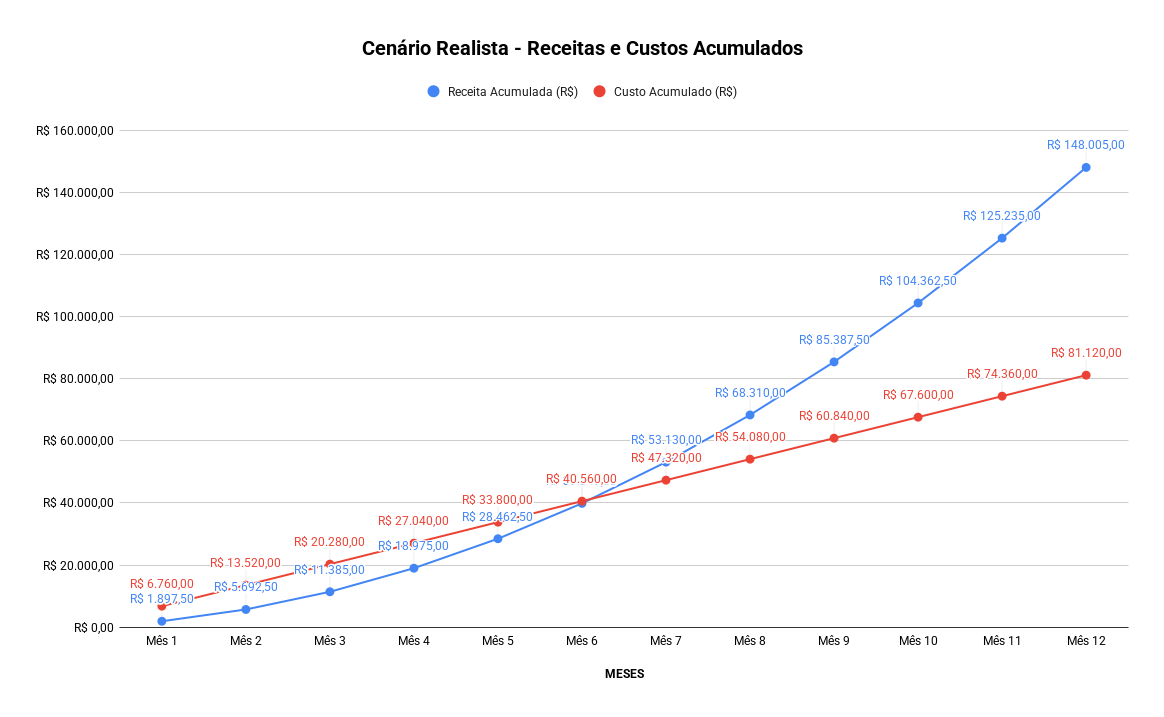
\includegraphics[width=0.9\textwidth]{cap05-viabilidade/imagens/cenario-realista.png}}
	\label{fig:cenario-realista}
	\fonte{Produzido pelos autores}
\end{figure}
\section{Cenário Otimista}

Texto
\section{Cenário Pessimista}

A Figura \ref{fig:cenario-pessimista} apresenta as receitas e custos acumulados no cenário pessimista considerando o projeto como um \gls{saas}. Nesse contexto, para o cálculo do acúmulo de receitas, estabeleceu-se um aumento mensal baixo de 5 clientes para o plano básico e 3 para o profissional.

Os custos consideram somente os gastos com mão de obra, infraestrutura e mensalidades ou licenças das ferramentas utilizadas no desenvolvimento e manutenção da aplicação.

No cenário pessismista, o ponto de equilíbrio não é atingido no doze meses de análise e, ao fim desse intervalo de tempo, há um prejuízo de R\$ 343 mil.
\begin{figure}[h]
	\centering
	\caption{Cenário pessimista}
	\fbox{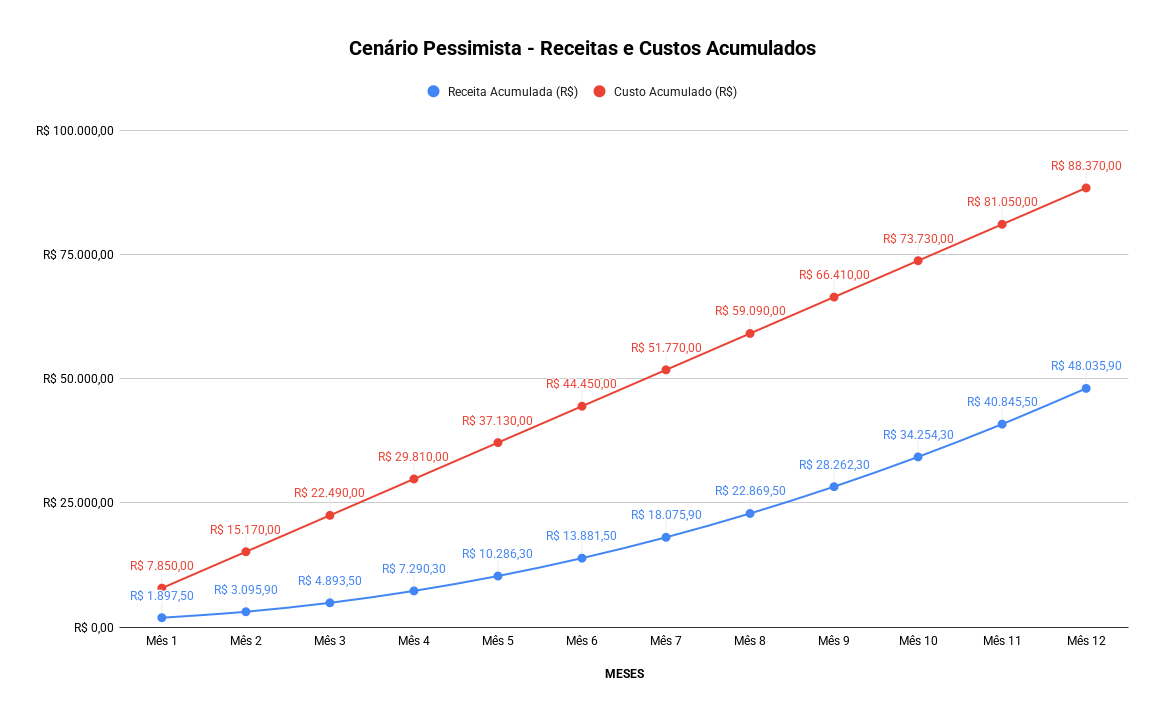
\includegraphics[width=0.9\textwidth]{cap05-viabilidade/imagens/cenario-pessimista.png}}
	\label{fig:cenario-pessimista}
	\fonte{Produzido pelos autores}
\end{figure}